%
%   Example for the inofficial Universität Passau LaTeX beamer style file.
%   ------
%
%   :copyright: (c) 2014 Philipp Jovanovic <philipp@jovanovic.io>.
%   :license: CC0, see LICENSE for more details.
%
\documentclass{beamer}

\usepackage{graphicx} % graphics
\usepackage{epsfig} % eps graphics
\usepackage{hyperref} % urls
\usepackage{caption} % custom captions
\usepackage[utf8x]{inputenc} % utf8 support

% suppress navigation bar
\beamertemplatenavigationsymbolsempty

\mode<presentation>
{
  \usetheme{unipassau}
  \setbeamercovered{transparent}
}
\logo{
\includegraphics[width=3cm]{logo.pdf}\vspace{218pt}\hspace{8pt}}


% title slide definition
\title[Short Title]{Title of the Presentation}
\subtitle{Subtitle}
\author{Author}
\institute[Fakultät]
{
  Fakultät\\
  Universität Passau\\
}
\date{Date}



%--------------------------------------------------------------------
%                            Titlepage
%--------------------------------------------------------------------

\begin{document}

\setbeamertemplate{footline}[default]

\section{Introduction}
\begin{frame}
  \titlepage
\end{frame}

%-------------------------------------------------------------------
%                            Content
%-------------------------------------------------------------------
% Set the footline with the custom theme.
\setbeamertemplate{footline}[unipassautheme]

\begin{frame}\frametitle{Frametitle 1}

  \begin{columns}[t]
  \column{5cm}
  \begin{block}{Definition}
  This is a definition.
  \end{block}
  \begin{itemize}
    \item Element 1
    \item Element 2
  \end{itemize}
  \begin{enumerate}
    \item Element 1
    \item Element 2
  \end{enumerate}
  \column{5cm}
  \begin{figure}
    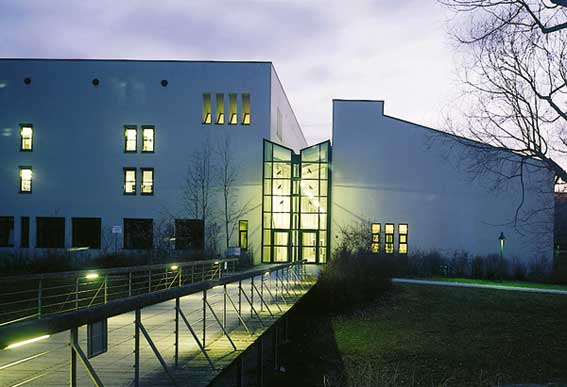
\includegraphics[width=5cm]{up.jpg}
    \caption{Universität Passau}
  \end{figure}
  \end{columns}

\end{frame}


\begin{frame}\frametitle{Frametitle 2}

  \begin{table}[ht!]
  \centering
  \begin{tabular}{|lccc|}
    \hline
    Name & Mat. Nr. & Semester & Degree Course \\
    \hline
    Example 1 & 1234 & 10 & M.Sc. BA\\
    Example 2 & 4567 &  8 & M.Sc. CS \\
    Example 3 & 7890 &  5 & B.A. ES \\
    Example 4 & 9012 &  4 & B.Sc. IC \\
    \hline
  \end{tabular}
  \caption{Students}
  \end{table}

\end{frame}


\end{document}
